% MechLens: BlackboxNLP 2026 revision of the ARR-reviewed manuscript

\documentclass[11pt]{article}
\usepackage[review]{acl}

\usepackage{times}
\usepackage{latexsym}
\usepackage[T1]{fontenc}
\usepackage[utf8]{inputenc}
\usepackage{microtype}
\usepackage{inconsolata}
\usepackage{graphicx}
\usepackage{amsmath}
\usepackage{amssymb}
\usepackage{booktabs}
\usepackage{multirow}
\usepackage{subcaption}
\usepackage{algorithm}
\usepackage{algorithmic}
\usepackage{xcolor}
\usepackage{tikz}
\usepackage{float}
\usepackage{stfloats}
\usepackage{url}
\usetikzlibrary{positioning,arrows.meta,shapes}

% ACL style handles hyperref internally

% Custom commands
\newcommand{\mechlens}{\textsc{MechLens}}
\newcommand{\rome}{\textsc{Rome}}
\newcommand{\memit}{\textsc{Memit}}
\newcommand{\iti}{\textsc{ITI}}
\newcommand{\dola}{\textsc{DoLa}}
\newcommand{\crystalboost}{\textsc{CrystalBoost}}
\newcommand{\caa}{\textsc{CAA}}

\title{\mechlens{}: Layerwise Factual Decodability Profiles \\
and Their Relationship to Intervention Effectiveness}

\author{
  Anonymous ACL submission
}

\begin{document}
\maketitle

% ==================== ABSTRACT ====================
\begin{abstract}
We study when correct factual answer tokens become explicitly decodable from language-model residual streams through vocabulary projections. We formalize this behavior with the \textbf{Factual Emergence Point (FEP)}, the earliest layer at which the answer enters the top-$k$ vocabulary predictions. Across five model families (Pythia, Gemma, Qwen2.5, Llama-3.1, and Mistral; 0.5--14B), 26.8\%--93.4\% of correct answers never enter the top-10 at an intermediate layer, and mean FEP occurs after 80\% of model depth. We call this empirical pattern \textbf{Late Crystallization}, referring specifically to late \emph{vocabulary-space decodability}, not to the location or first causal use of factual knowledge. Tuned-lens, top-$k$ sensitivity, cross-benchmark, and sentiment-control experiments test the robustness and scope of this measurement.

We further compare these decodability profiles with factuality interventions. \caa{} outperforms \dola{} on Llama and Mistral ($p{<}0.001$), whereas \dola{} is directionally better on Qwen (+25.4\% vs.\ +15.5\% MC1; two-sided $p{=}0.069$). We therefore present crystallization degree as an \emph{exploratory diagnostic association}, rather than a validated universal selection rule. Additional results include a category-level Computability--Memorization pattern, a LayerNorm intervention (+11.8\% MC1), and open-source \mechlens{} tooling for five model families.\footnote{Code: \url{https://anonymous.4open.science/r/MechLens-EMNLP2026}}
\end{abstract}

% ==================== 1. INTRODUCTION ====================
\section{Introduction}
\label{sec:introduction}

\begin{figure}[H]
    \centering
    \resizebox{\columnwidth}{!}{
    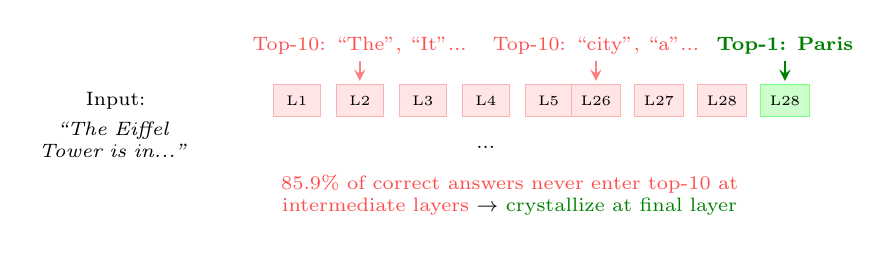
\begin{tikzpicture}[
        layer/.style={rectangle, draw=gray!50, fill=gray!10, minimum width=0.6cm, minimum height=0.4cm, font=\tiny},
        invisible/.style={rectangle, draw=red!30, fill=red!10, minimum width=0.6cm, minimum height=0.4cm, font=\tiny},
        visible/.style={rectangle, draw=green!50, fill=green!20, minimum width=0.6cm, minimum height=0.4cm, font=\tiny},
        arrow/.style={->, >=stealth, thick},
        label/.style={font=\scriptsize}
    ]
    % Input
    \node[label] at (-1.5, 0) {Input:};
    \node[label, text width=2cm, align=center] at (-1.5, -0.5) {\textit{``The Eiffel Tower is in...''}};
    
    % Layers
    \foreach \i in {1,...,5} {
        \node[invisible] (l\i) at (\i*0.8, 0) {L\i};
    }
    \node[label] at (3.2, -0.6) {...};
    \foreach \i in {6,...,8} {
        \node[invisible] (l\i) at (\i*0.8-0.2, 0) {L\the\numexpr\i+20\relax};
    }
    \node[visible] (lN) at (7.0, 0) {L28};
    
    % Top prediction labels
    \node[label, red!70] at (1.6, 0.7) {Top-10: ``The'', ``It''...};
    \node[label, red!70] at (4.6, 0.7) {Top-10: ``city'', ``a''...};
    \node[label, green!50!black] at (7.0, 0.7) {\textbf{Top-1: Paris}};
    
    % Arrows
    \draw[arrow, red!50] (1.6, 0.5) -- (1.6, 0.25);
    \draw[arrow, red!50] (4.6, 0.5) -- (4.6, 0.25);
    \draw[arrow, green!50!black, thick] (7.0, 0.5) -- (7.0, 0.25);
    
    % Caption below
    \node[label, text width=8cm, align=center] at (3.5, -1.2) {
        \textcolor{red!70}{85.9\% of correct answers never enter top-10 at intermediate layers} $\rightarrow$ \textcolor{green!50!black}{crystallize at final layer}
    };
    \end{tikzpicture}
    }
    \caption{\textbf{Late Crystallization}: correct answer tokens remain outside the top vocabulary predictions at intermediate layers and become explicitly decodable only near the output.}
    \label{fig:concept}
\end{figure}

Large language models (LLMs) frequently produce plausible-sounding but factually incorrect outputs---hallucinations---posing significant challenges for deployment in high-stakes applications \citep{huang2023survey,ji2023survey}. A natural approach to mitigating hallucinations is to characterize how factual information is processed and when candidate answers become readable from internal representations. This requires separating evidence about \emph{vocabulary-space readout} from stronger claims about where knowledge is stored or causally used.

Prior work on knowledge localization has produced mixed evidence. Causal tracing \citep{meng2022locating} identifies middle-layer MLPs as critical for factual recall in GPT-2, motivating localized editing methods like ROME and MEMIT. However, recent work suggests knowledge may be more distributed than initially assumed \citep{geva2022transformer}, raising questions about whether activation-level interventions can effectively modulate factual behavior.

We introduce \mechlens{}, a unified interpretability framework for systematic analysis of these questions. Through logit-lens analysis, layer contrasting, and activation interventions across \textbf{five} model families, we quantify \textbf{Late Crystallization}: correct factual answer tokens often become vocabulary-decodable only near the output (Figure~\ref{fig:concept}). Our contributions are:

\begin{itemize}
    \item \textbf{Systematic quantification}: FEP occurs after 80\% of depth across the tested models; strict final-layer rates vary from 26.8\% to 93.4\%. The trend is evaluated across model families, scales, benchmarks, vocabulary-projection methods, and $k$ thresholds.
    \item \textbf{Scope and controls}: On models that perform zero-shot SST-2, answer-token decodability is substantially earlier for sentiment classification than for factual retrieval, indicating that late FEP is not a generic property of all next-token decisions.
    \item \textbf{Intervention association}: \caa{} and \dola{} exhibit different cross-model effectiveness patterns. We report this as an exploratory association with crystallization degree and make explicit the small model-level sample and non-significant two-sided Qwen comparison.
    \item \textbf{Representation analyses}: Head ablations are diffuse at the FEP boundary (Gini$<$0.015), while LayerNorm ablation leaves FEP unchanged. These results constrain, but do not identify, the mechanism producing late vocabulary-space readout.
    \item \textbf{Category-level pattern}: Categories labeled as more computable have earlier FEP than categories dominated by factual recall, motivating further tests of a Computability--Memorization hypothesis.
\end{itemize}

Together, these results provide a measurement framework for studying when factual answers become vocabulary-decodable and how those profiles relate to intervention behavior.

% ==================== 2. RELATED WORK ====================
\section{Related Work}
\label{sec:related}

\paragraph{Knowledge Localization and Editing.}
Causal tracing \citep{meng2022locating} identifies middle-layer MLPs as critical for factual recall in GPT-2, motivating ROME and MEMIT \citep{meng2022mass}. \citet{geva2021transformer,geva2022transformer} show that MLPs promote factual concepts, and \citet{geva2023dissecting} describe subject enrichment, relation propagation, and late attribute extraction. \citet{nanda2023factfinding} similarly identifies late components involved in moving answer information to the final token position. These results make late answer-token visibility plausible; our contribution is not the discovery that predictions sharpen with depth, but a population-level metric and cross-model quantification of \emph{when} answers enter the vocabulary ranking. Logit lens \citep{nostalgebraist2020logitlens} and tuned lens \citep{belrose2023tuned} provide the relevant projections, while concurrent work \citep{wang2025logitlens4llms} reports late-layer concentration in modern architectures. Table~\ref{tab:prior_work} summarizes the empirical scope added here.

Late FEP is also distinct from \emph{grokking} \citep{power2022grokking}. Grokking describes delayed generalization over training time after overfitting on algorithmic datasets; FEP instead measures how answer-token decodability changes across depth in a fixed pretrained model during one forward pass. The visual analogy of a late transition therefore does not imply a shared mechanism.

\begin{table}[t]
\centering\small
\resizebox{\columnwidth}{!}{
\begin{tabular}{lcc}
\toprule
& \textbf{Prior Work} & \textbf{This Work} \\
\midrule
Observation & Qualitative & \textbf{Quantified} (85.9\%) \\
Metric & Implicit & \textbf{FEP} (formal) \\
Cross-arch & Limited & \textbf{5 architectures} \\
Causal/readout link & Circuit cases & \textbf{50-example comparison} \\
Intervention link & Indirect & \textbf{Exploratory association} \\
\bottomrule
\end{tabular}
}
\caption{Comparison with prior logit lens studies.}
\label{tab:prior_work}
\end{table}

\paragraph{Activation Intervention for Factual Accuracy.}
\iti{} \citep{li2023inference} shifts activations along probed truthfulness directions. \dola{} \citep{chuang2024dola} contrasts early/late logit distributions without learned directions. \caa{} \citep{turner2023activation} and representation engineering \citep{zou2023representation} steer via contrastive activation vectors. SADI \citep{zhang2025sadi} achieves state-of-the-art MC1=67\% via semantic-adaptive intervention on instruction-tuned models. CCS \citep{burns2022discovering} discovers latent knowledge through consistency constraints. These methods operate in activation space (\iti{}, \caa{}, SADI) or logit space (\dola{}); we test whether their effectiveness covaries with layerwise vocabulary-decoding profiles.

% ==================== 3. MECHLENS FRAMEWORK ====================
\section{The \mechlens{} Framework}
\label{sec:framework}

\mechlens{} is built on TransformerLens \citep{nanda2022transformerlens} and supports five model families spanning diverse architectures: Pythia \citep{biderman2023pythia}, Gemma \citep{gemma2024}, Qwen2.5 \citep{qwen2024qwen25}, Llama-3.1 \citep{dubey2024llama3}, and Mistral \citep{jiang2023mistral} (Table~\ref{tab:models}).

\begin{table}[t]
\centering
\small
\resizebox{\columnwidth}{!}{
\begin{tabular}{lcccl}
\toprule
\textbf{Model} & \textbf{Layers} & \textbf{Heads} & \textbf{$d$} & \textbf{Attention} \\
\midrule
Qwen2.5-0.5B & 24 & 14 & 896 & GQA (2 KV) \\
Qwen2.5-7B & 28 & 28 & 3584 & GQA (4 KV) \\
Qwen2.5-14B & 48 & 40 & 5120 & GQA (8 KV) \\
Pythia-1.4B & 24 & 16 & 2048 & MHA \\
Pythia-6.9B & 32 & 32 & 4096 & MHA \\
Llama-3.1-8B & 32 & 32 & 4096 & GQA (8 KV) \\
Mistral-7B & 32 & 32 & 4096 & GQA+SWA (8 KV) \\
Gemma-7B & 28 & 16 & 3072 & MHA \\
\bottomrule
\end{tabular}
}
\caption{Supported model architectures. Qwen2.5-14B enables cross-scale validation (\S\ref{sec:scale}).}
\label{tab:models}
\end{table}

\paragraph{Analysis.} We extend causal tracing \citep{meng2022locating} with adaptive noise calibration ($\sigma = \alpha \cdot \text{std}(\mathbf{E}(x))$, $\alpha{=}10$), KL divergence metrics, and multi-run averaging ($n{=}5$). We also implement contrastive activation analysis, computing normalized L2 distance between correct and hallucinated residual stream activations at each layer. Full methodological details are in Appendix~\ref{app:methods}.

\paragraph{Intervention.} \mechlens{} supports three reversible intervention types through hooks: ablation ($\mathbf{h}'_{l,c} = \mathbf{0}$), scaling ($\mathbf{h}'_{l,c} = \alpha \cdot \mathbf{h}_{l,c}$), and injection ($\mathbf{h}'_{l,c} = \mathbf{h}^{\text{source}}_{l,c}$). For \caa{}, we follow \citet{turner2023activation}: given paired truthful/untruthful prompts, we extract contrastive directions $\mathbf{d}_l = \frac{1}{N}\sum_i(\mathbf{h}_l(x^+_i) - \mathbf{h}_l(x^-_i))$ and add $\alpha \cdot \mathbf{d}_l$ to the top-$k$ layers ranked by $\|\mathbf{d}_l\|_2$ at inference time. Directions are extracted from 256 TruthfulQA training pairs.

% ==================== 4. EXPERIMENTAL SETUP ====================
\section{Experimental Setup}
\label{sec:setup}

\paragraph{Models and Phases.} \emph{Phase~1} (causal tracing, contrastive analysis, activation scaling) uses Qwen2.5-0.5B and Pythia-1.4B---matched 24-layer models with different architectures (GQA/SwiGLU vs.\ MHA/GELU). \emph{Phase~2} (FEP detection, MC1/MC2 evaluation, cross-architecture validation) uses Qwen2.5-7B, Llama-3.1-8B, and Mistral-7B on the full TruthfulQA benchmark (817 samples) \citep{lin2022truthfulqa}. \emph{Phase~3} (cross-scale validation) extends FEP detection to Qwen2.5-14B (48 layers) to test whether Late Crystallization persists at larger scale.

\paragraph{Evaluation.} Phase~1 screening uses 200 TruthfulQA samples with keyword matching plus LLM-as-Judge \citep{zheng2024judging}. Phase~2 uses standardized MC1 (single-correct accuracy) and MC2 (normalized probability mass) on all 817 samples. We test 20 activation scaling strategies across 6 categories plus an 18-configuration ITI grid search; full details and results are in Appendix~\ref{app:negative_results}.

% ==================== 5. RESULTS ====================
\section{Results}
\label{sec:results}

\subsection{Negative Results: Activation Scaling and ITI}
\label{sec:negative_results}

Simple activation scaling fails to provide a meaningful gain across the 20 tested strategy--model settings ($\leq$2\% gain; up to 28\% degradation), and an 18-configuration ITI grid search achieves at most +2\%. This broad negative result motivates analysis of layerwise decodability (\S\ref{sec:crystallization}; full tables in Appendix~\ref{app:negative_results}).

\subsection{MC1/MC2 Evaluation with Advanced Interventions}
\label{sec:mc_results}

We evaluate four methods on the full 817-sample TruthfulQA benchmark using Qwen2.5-7B (Table~\ref{tab:mc_results}).

\begin{table}[t]
\centering
\small
\begin{tabular}{llcc}
\toprule
\textbf{Method} & \textbf{Configuration} & \textbf{MC1} & \textbf{MC2} \\
\midrule
Baseline & --- & 0.2215 & 0.3921 \\
\midrule
\iti{} & top\_k=3, $\lambda$=1--3 & 0.2215 & 0.3921 \\
\iti{} & top\_k=5, $\lambda$=1--3 & 0.2203 & 0.3926 \\
\iti{} & top\_k=10, $\lambda$=3 & \textbf{0.2436} & \textbf{0.4178} \\
\midrule
\dola{} & early (static) & 0.2326 & 0.4371 \\
\dola{} & mid (static) & 0.2448 & 0.4555 \\
\dola{} & dynamic & \textbf{0.2778} & \textbf{0.4822} \\
\midrule
\caa{} & top\_k=3, all coeff & 0.2215 & 0.3921 \\
\caa{} & top\_k=5, all coeff & 0.2203 & 0.3922 \\
\caa{} & top\_k=10, coeff=5.0 & \textbf{0.2558} & \textbf{0.4338} \\
\bottomrule
\end{tabular}
\caption{MC1/MC2 on TruthfulQA (Qwen2.5-7B, 817 samples). \dola{} dynamic achieves the best MC1 (+25.4\% over baseline, $p{=}0.009$). 95\% bootstrap CI for MC1 $\approx \pm 0.03$ ($n{=}817$).}
\label{tab:mc_results}
\end{table}

\paragraph{Key findings.} A clear hierarchy emerges: \dola{} dynamic (+25.4\% MC1) $>$ \caa{} top\_k=10 (+15.5\%) $>$ \iti{} top\_k=10 (+10.0\%) $>$ simple scaling (0\%). Both \iti{} and \caa{} show \emph{zero} improvement at top\_k$\in\{3,5\}$ but substantial gains at top\_k=10, indicating a layer-count threshold. That \dola{} (logit-space) achieves the largest gains motivates our mechanistic analysis in Section~\ref{sec:crystallization}. All experiments use base (non-instruction-tuned) models (MC1 baselines: 18.9--22.2\%); absolute values should not be compared with instruction-tuned methods like SADI \citep{zhang2025sadi} (MC1=67\%). \dola{}'s improvement is significant (two-proportions $z$-test: $z{=}2.63$, $p{=}0.009$; survives Bonferroni correction at $\alpha{=}0.017$).

% ==================== 6. LATE CRYSTALLIZATION ====================
\section{Late Vocabulary-Space Decodability}
\label{sec:crystallization}

The effectiveness hierarchy observed in Section~\ref{sec:mc_results} motivates a closer measurement of layerwise answer readout. We use \textbf{Late Crystallization} as shorthand for an empirical pattern in which the correct answer enters the vocabulary ranking only near the output. The term does not imply that the underlying factual representation is first stored or causally used at that layer.

\subsection{Factual Emergence Point Detection}
\label{sec:fep}

We define the \textbf{Factual Emergence Point (FEP)} for a query $q$ with correct answer $a$ as the earliest layer $L$ at which $a$ enters the top-$k$ predictions under logit lens projection:
\begin{equation}
    L_{\text{FEP}} = \min\{L : \text{rank}(a, \mathbf{W}_U \cdot \text{LN}(\mathbf{h}_L)) \leq k\}
\end{equation}
where $\mathbf{h}_L$ is the residual stream at layer $L$, LN is the final layer norm, and $\mathbf{W}_U$ is the unembedding matrix. If $a$ never enters top-$k$ at any intermediate layer, we set $L_{\text{FEP}} = L_{\max}$ (the final layer). We use $k=10$ throughout.

FEP concerns \emph{vocabulary-space readout}. It is distinct from representation---information encoded in activations that may support downstream computation---and storage---the parameters or modules encoding a factual association. To test this distinction directly, causal tracing on 50 Qwen2.5-7B TruthfulQA examples places the mean causal peak at layer 1.1/28 but the mean FEP at 27.7/28; 47/50 examples combine an early causal peak with late FEP. Thus, early causal involvement and late vocabulary decodability can coexist.

\paragraph{Tuned lens validation.} A natural concern is that FEP${}=L_{\max}$ for 85.9\% of samples could reflect logit lens's known limitations. We train per-layer affine probes on 2{,}000 WikiText-2 samples and compute tuned-lens FEP on all 817 TruthfulQA samples: the tuned lens yields 85.7\% strict final-layer FEP---within 0.2 percentage points of the logit lens (85.9\%)---with 74.9\% of samples having identical FEP (Table~\ref{tab:tuned_lens}). This agreement reduces sensitivity to the choice between these two vocabulary projections, but neither probe establishes knowledge absence or localization.

\begin{table}[t]
\centering\small
\resizebox{\columnwidth}{!}{
\begin{tabular}{lcccc}
\toprule
\textbf{Probe} & \textbf{Mean FEP} & \textbf{Late Crystal} & \textbf{Exact Match} & \textbf{$\pm$2 Match} \\
\midrule
Logit lens & 27.3$\pm$1.8 & 85.9\% & \multirow{2}{*}{74.9\%} & \multirow{2}{*}{76.4\%} \\
Tuned lens & 25.1$\pm$7.4 & 85.7\% & & \\
\bottomrule
\end{tabular}
}
\caption{Tuned lens vs.\ logit lens FEP (Qwen2.5-7B, 817 samples). Both yield near-identical late crystallization rates ($\Delta$=0.2\%).}
\label{tab:tuned_lens}
\end{table}

We compute FEP for all 817 TruthfulQA samples on Qwen2.5-7B (28 layers), tracking the rank of each correct answer's first token across all layers via logit lens projection.

\paragraph{Robustness to $k$ threshold.} Late Crystallization is robust across $k \in \{1, 3, 5, 10, 20, 50, 100\}$: even at $k{=}100$ (top 0.1\% of vocabulary), 64.7\% of correct answers still never appear at any intermediate layer, and FEP Depth remains above 93\% (Table~\ref{tab:topk_sensitivity} in Appendix~\ref{app:topk}).

\subsection{The Late Crystallization Phenomenon}

Table~\ref{tab:fep_distribution} reveals a striking pattern: \textbf{85.9\% of correct answers (702/817) never enter the top-10 predictions at any intermediate layer} (mean FEP = 27.3 $\pm$ 1.8 out of 28 layers). This \textbf{Late Crystallization} result establishes late answer-token visibility under vocabulary projection. It remains compatible with factual information being represented and causally processed at earlier layers.

\begin{table}[t]
\centering
\small
\begin{tabular}{lrr}
\toprule
\textbf{FEP Layer} & \textbf{Count} & \textbf{Percentage} \\
\midrule
28 (final / never) & 702 & 85.9\% \\
23 & 47 & 5.8\% \\
21 & 20 & 2.4\% \\
25 & 13 & 1.6\% \\
Other ($\leq$1.2\% each) & 35 & 4.3\% \\
\bottomrule
\end{tabular}
\caption{FEP distribution (Qwen2.5-7B, 817 TruthfulQA samples). 85.9\% of correct answers \emph{never} enter top-10 at any intermediate layer.}
\label{tab:fep_distribution}
\end{table}

\subsection{Computability--Memorization Spectrum}
\label{sec:spectrum}

FEP varies systematically across knowledge categories (full table in Appendix~\ref{app:spectrum}): Logical Falsehood has the earliest mean FEP (22.1, $\sigma$=2.6), while History, Psychology, and Weather have FEP=28.0 with zero variance. We refer to this descriptive gradient as a \textbf{Computability--Memorization Spectrum}. Because these category labels are proxies rather than controlled measures of computation or memorization, we treat the proposed interpretation as a hypothesis for future validation.

\subsection{FEP--\dola{} Decorrelation}
\label{sec:fep_dola}

\dola{}'s dynamic layer selection does not correlate with FEP (Pearson $r = -0.057$, $p = 0.103$): \dola{} selects near-exclusively layer 0--1 (mean = 0.95), while FEP concentrates at layer 27--28. This is consistent with \dola{} contrasting pre- and post-readout vocabulary distributions rather than selecting the exact FEP layer. Likewise, \caa{}/\iti{} improve only when applied across at least ten layers in our search. These observations motivate, but do not causally establish, a connection between decodability profiles and intervention behavior.

% ==================== 7. CROSS-ARCHITECTURE VALIDATION ====================
\section{Cross-Architecture Validation and Analysis}
\label{sec:cross_arch}

We extend our analysis to four additional architectures: Llama-3.1-8B (GQA), Mistral-7B (GQA+SWA), Pythia-6.9B (standard MHA), and Gemma-7B (standard MHA), covering the major attention mechanism variants.

\subsection{Cross-Architecture FEP Detection}

\begin{table}[t]
\centering
\small
\resizebox{\columnwidth}{!}{
\begin{tabular}{lcccc}
\toprule
\textbf{Model} & \textbf{Layers} & \textbf{Mean FEP} & \textbf{FEP Depth} & \textbf{Late Crystal} \\
\midrule
Qwen2.5-7B & 28 & 27.3 $\pm$ 1.8 & 97.5\% & 85.9\% \\
Qwen2.5-14B & 48 & 46.0 $\pm$ 4.9 & 95.8\% & 77.7\% \\
Llama-3.1-8B & 32 & 29.4 $\pm$ 4.9 & 91.9\% & 71.0\% \\
Mistral-7B & 32 & 26.3 $\pm$ 6.2 & 82.3\% & 27.1\% \\
Pythia-6.9B & 32 & 30.8 $\pm$ 4.2 & 96.2\% & 93.4\% \\
Gemma-7B & 28 & 27.4 $\pm$ 2.4 & 97.7\% & 89.8\% \\
\bottomrule
\end{tabular}
}
\caption{Cross-architecture and cross-scale FEP detection (817 samples). FEP Depth = Mean FEP / total layers. All tested models show mean answer-token decodability after 80\% depth, with substantial variation in strict final-layer FEP.}
\label{tab:cross_fep}
\end{table}

Table~\ref{tab:cross_fep} and Figure~\ref{fig:fep_heatmap} show two empirical trends: (1) mean FEP occurs after 80\% model depth for every tested model (range: 82.2\%--97.7\%); and (2) strict final-layer FEP ranges from 93.4\% for Pythia to 26.8\% for Mistral. Because model family, training data, tokenizer, attention type, and head configuration vary jointly, these comparisons do not isolate an architectural cause. In particular, Mistral's sliding-window attention is one possible factor rather than an established explanation.

\subsection{Cross-Scale Validation (Qwen2.5-14B)}
\label{sec:scale}

To examine scaling within one family, we run FEP detection on Qwen2.5-14B (48 layers, 14.7B parameters). Here, 77.7\% of correct answers never enter the top-10 at an intermediate layer, and FEP Depth is 95.8\% (vs.\ 97.5\% at 7B). This two-point comparison suggests stability within Qwen2.5 from 7B to 14B; it is not sufficient to establish scale invariance more broadly.

\subsection{Cross-Benchmark Validation (MMLU)}
\label{sec:mmlu}

To test whether the measurement extends beyond TruthfulQA, we run FEP detection on 1{,}200 MMLU samples spanning 24 subjects. Strict final-layer FEP reaches 98.2\%, with similar rates across STEM (99.1\%), Humanities (98.0\%), Social Sciences (97.2\%), and Other (98.0\%) domains (Table~\ref{tab:mmlu_fep} in Appendix~\ref{app:mmlu}). This cross-benchmark result establishes a second multiple-choice setting; explaining the higher MMLU rate requires controlled analysis beyond the present data.

\begin{figure*}[t]
    \centering
    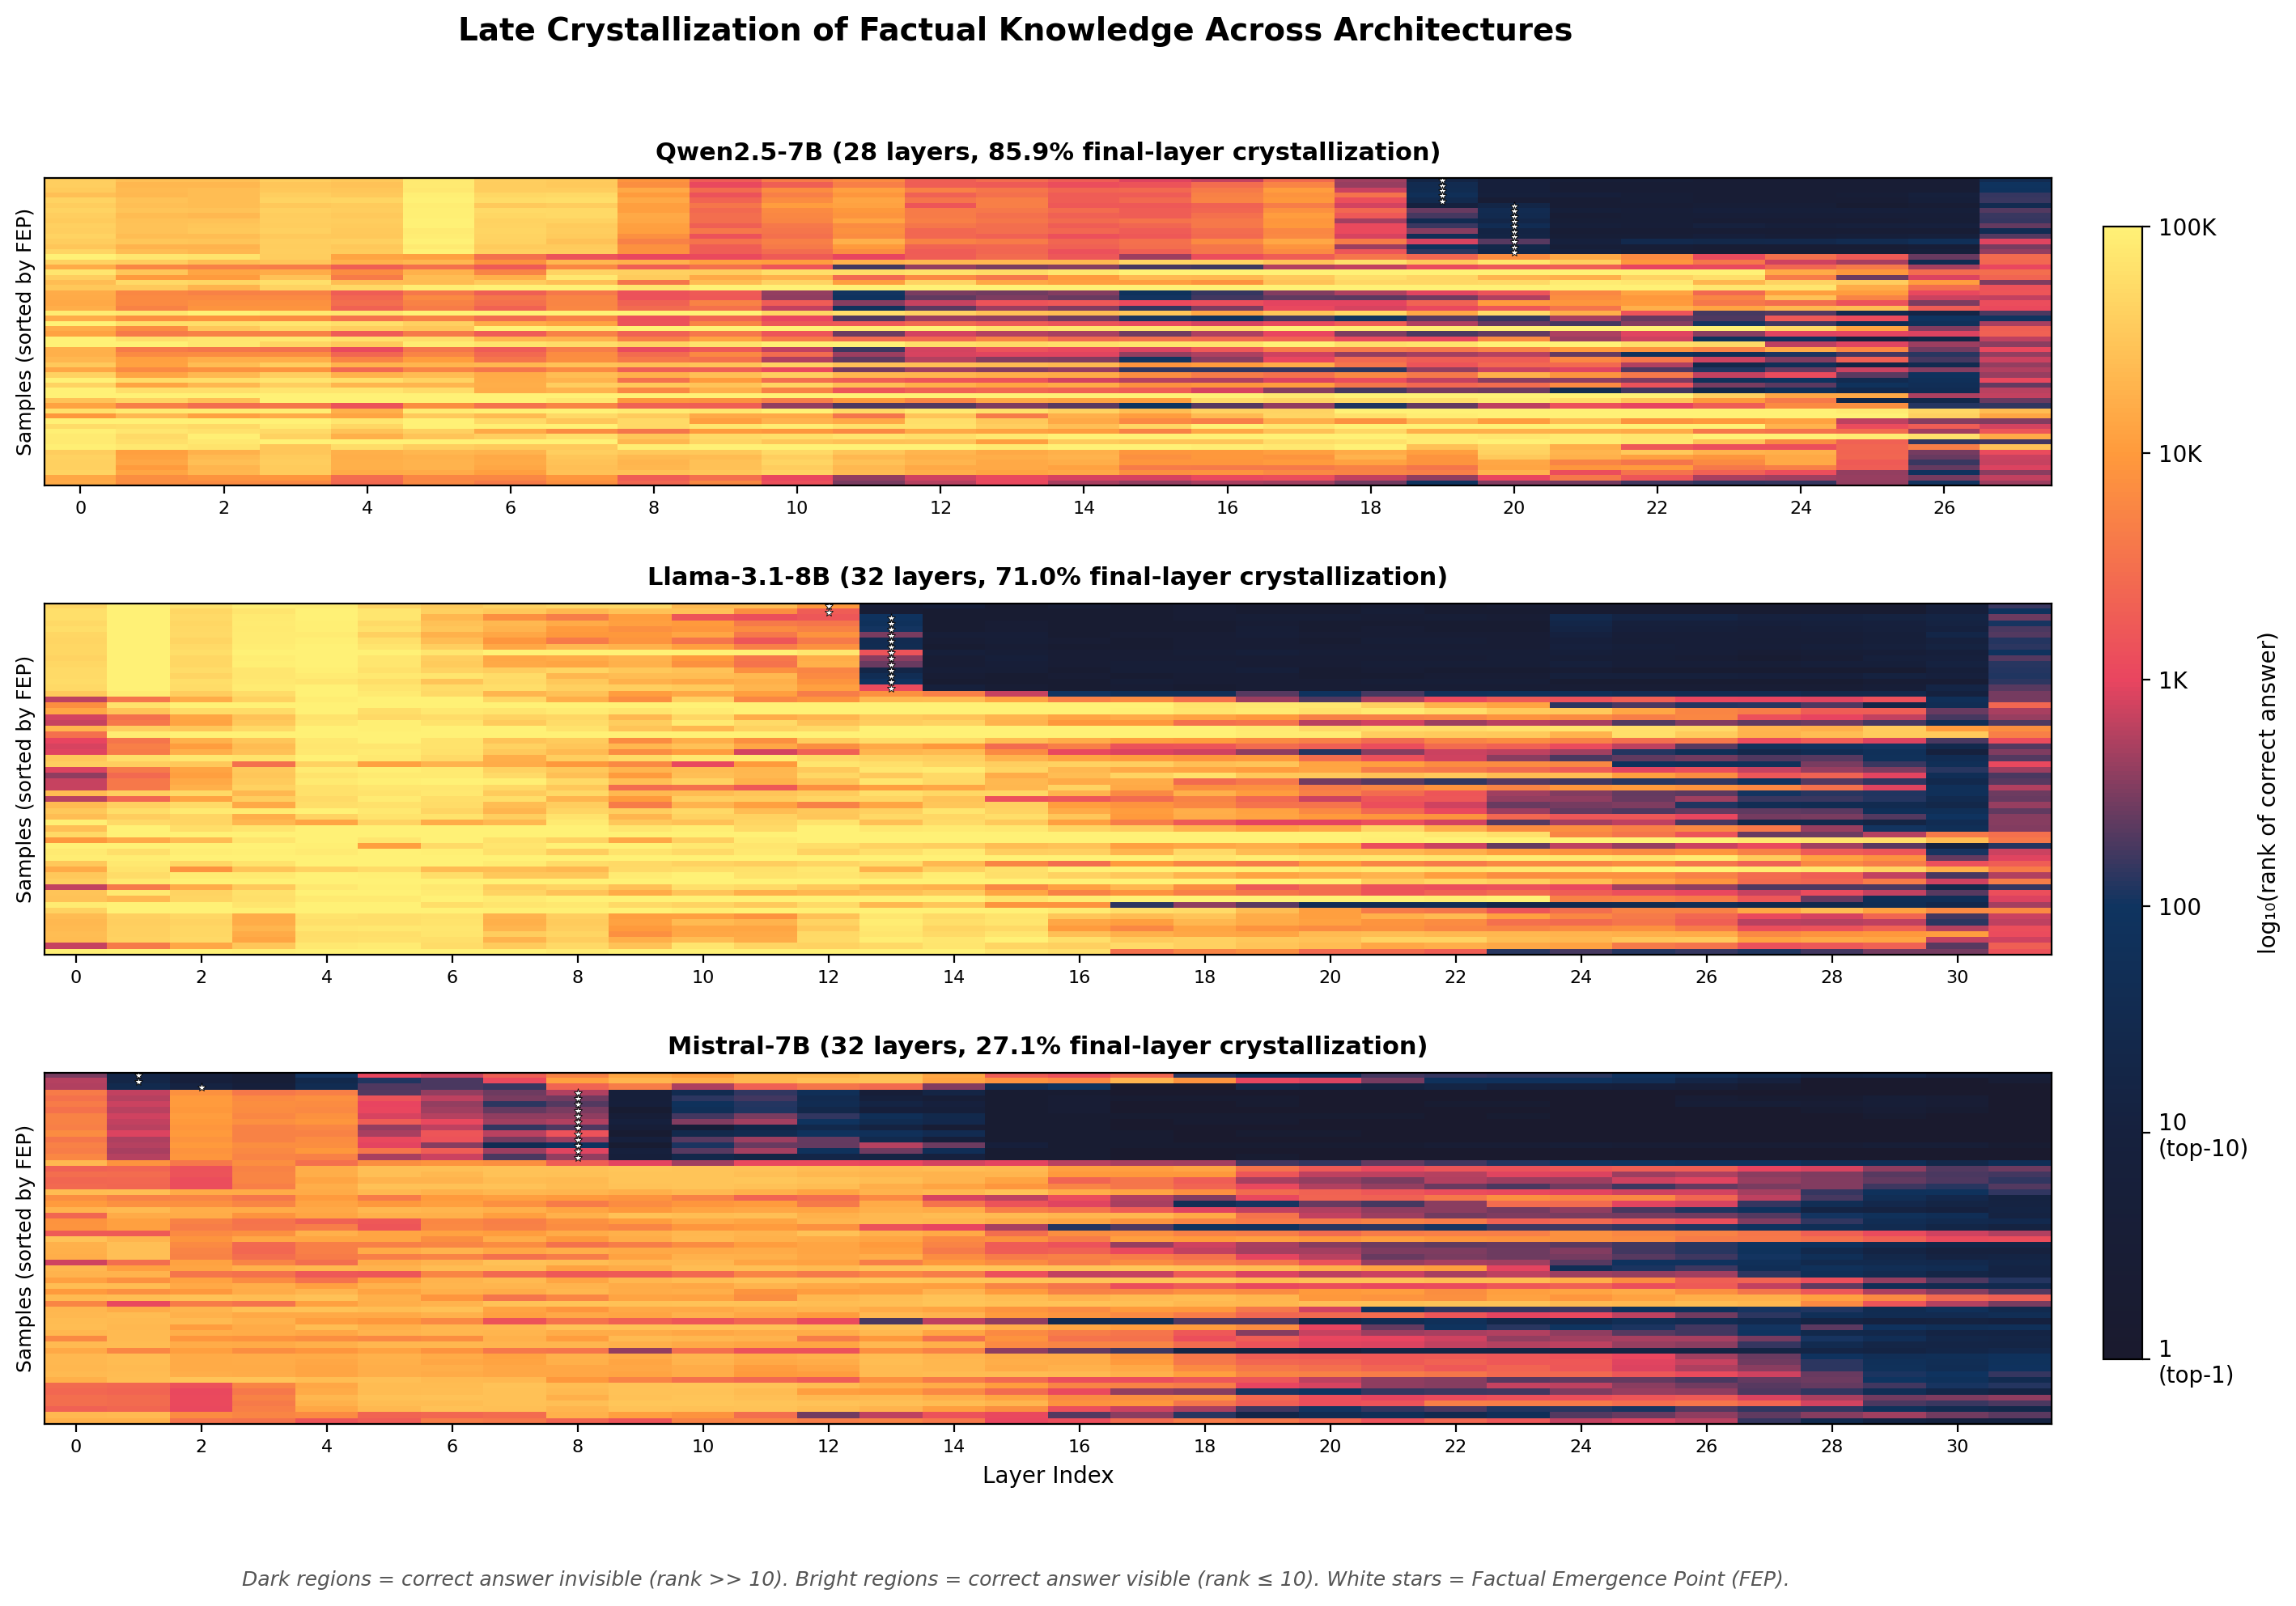
\includegraphics[width=\textwidth]{figures/fep_crystallization_heatmap.png}
    \caption{Late Crystallization across architectures. Each row: a TruthfulQA sample; each column: a layer. Color: $\log_{10}(\text{rank})$ of correct answer under logit lens. White stars: FEP.}
    \label{fig:fep_heatmap}
\end{figure*}

\begin{figure*}[t]
    \centering
    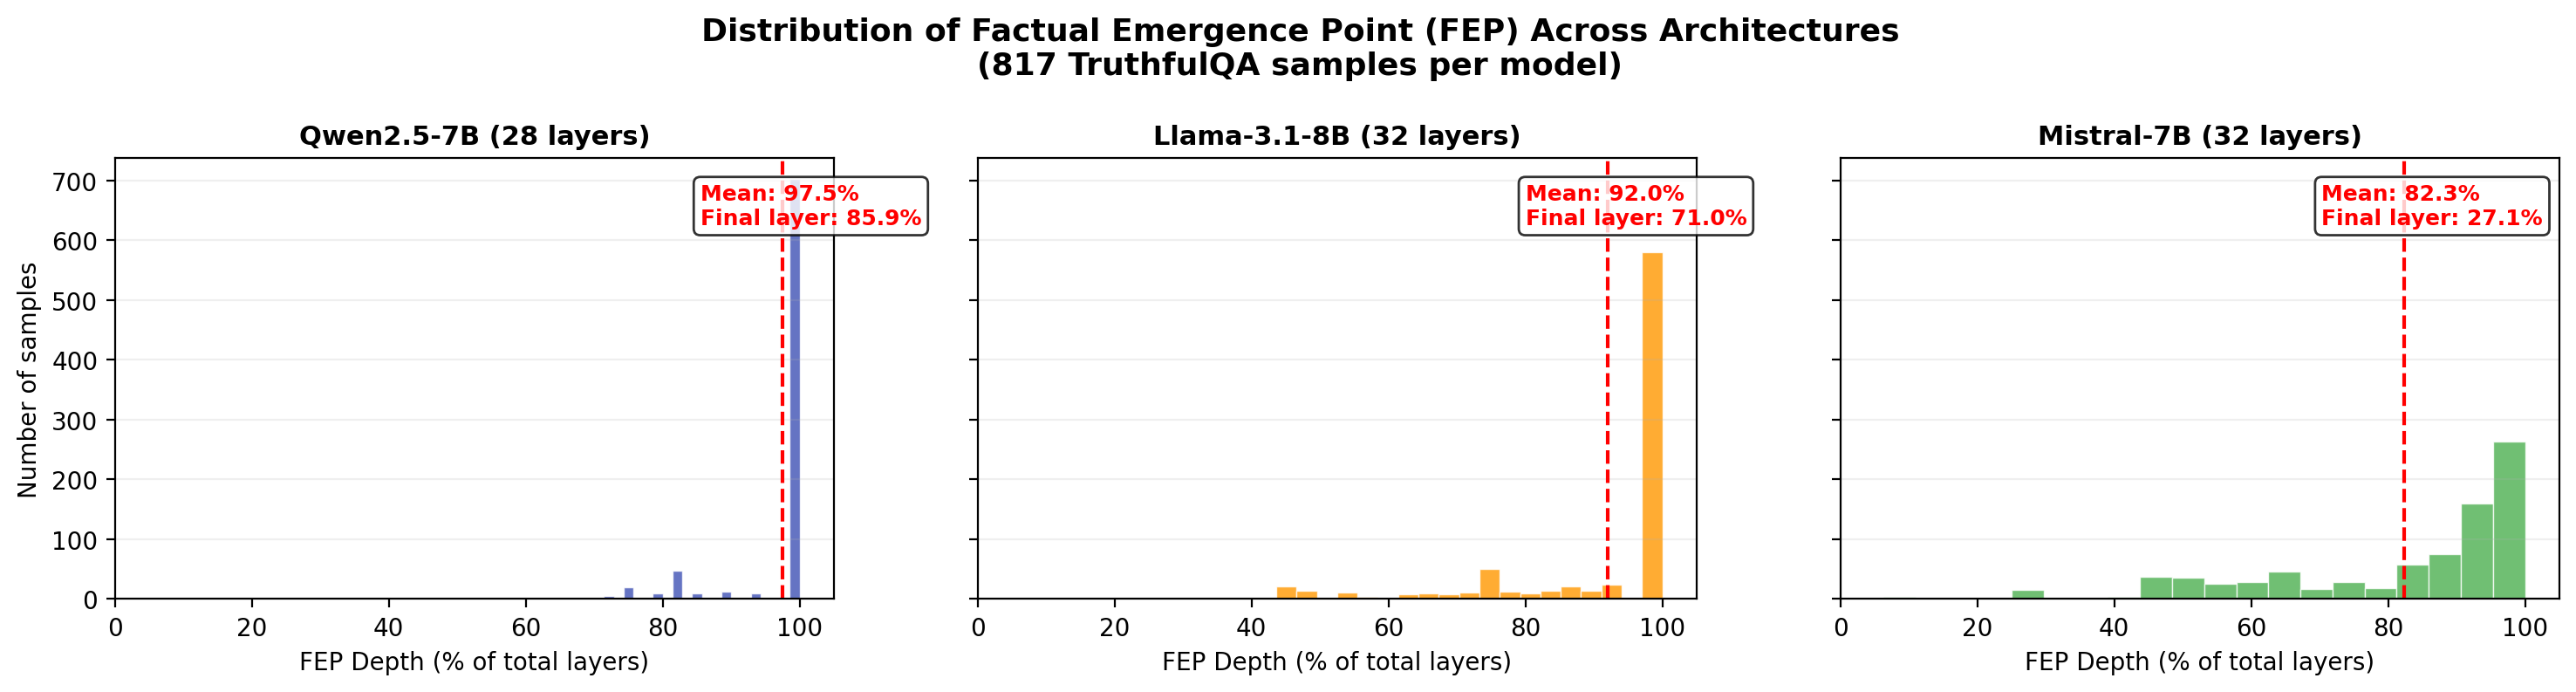
\includegraphics[width=0.9\textwidth]{figures/fep_distribution_comparison.png}
    \caption{FEP depth distribution across architectures (817 samples each). Qwen concentrates at the final layer (85.9\%), Llama shows a bimodal pattern (71.0\%), Mistral distributes broadly (27.1\%) while maintaining $>$82\% mean depth.}
    \label{fig:fep_dist}
\end{figure*}

\subsection{Association with Intervention Effectiveness}

\begin{table}[t]
\centering
\small
\begin{tabular}{llcc}
\toprule
\textbf{Model} & \textbf{Method} & \textbf{MC1} & \textbf{$\Delta$\%} \\
\midrule
\multirow{3}{*}{Llama-3.1-8B} & Baseline & 0.1897 & --- \\
 & \dola{} dynamic & 0.1934 & $+1.9$ \\
 & \caa{} (top\_k=10) & \textbf{0.2534} & $\mathbf{+33.5}$ \\
\midrule
\multirow{3}{*}{Mistral-7B} & Baseline & 0.2044 & --- \\
 & \dola{} dynamic & 0.2277 & $+11.4$ \\
 & \caa{} (top\_k=10) & \textbf{0.2705} & $\mathbf{+32.3}$ \\
\midrule
\multirow{3}{*}{Qwen2.5-7B} & Baseline & 0.2215 & --- \\
 & \dola{} dynamic & \textbf{0.2778} & $\mathbf{+25.4}$ \\
 & \caa{} (top\_k=10) & 0.2558 & $+15.5$ \\
\bottomrule
\end{tabular}
\caption{Cross-architecture intervention results (817 samples). \caa{} outperforms \dola{} on Llama and Mistral; \dola{} is directionally better on Qwen, but the two-sided Qwen comparison is not significant ($p{=}0.069$).}
\label{tab:cross_interventions}
\end{table}

Table~\ref{tab:cross_interventions} shows an exploratory cross-model association. \caa{} outperforms \dola{} on Llama (+33.5\% vs.\ +1.9\%; $p{<}0.001$) and Mistral (+32.3\% vs.\ +11.4\%; $p{=}0.001$), with both comparisons surviving Bonferroni correction ($\alpha{=}0.017$). On Qwen, \dola{} is directionally better (+25.4\% vs.\ +15.5\%), but the two-sided comparison is not significant ($p{=}0.069$). A paired re-evaluation on all 817 examples gives one-tailed bootstrap $p{=}0.038$ and McNemar $p{=}0.045$ under the directional hypothesis stated before that analysis. Because only three model families have matched intervention comparisons and the Qwen conclusion depends on a directional test, we do not claim a universal threshold or a validated method-selection rule. The pattern instead motivates broader controlled evaluation of decodability profiles as a diagnostic variable.

\subsection{LayerNorm Ablation Analysis}
\label{sec:ln_ablation}

To test whether final LayerNorm is necessary for the measured pattern, we ablate and scale ln\_final on Qwen2.5-7B (Table~\ref{tab:ln_ablation}).

\begin{table}[t]
\centering
\small
\resizebox{\columnwidth}{!}{
\begin{tabular}{lcccc}
\toprule
\textbf{Condition} & \textbf{Mean FEP} & \textbf{Late Crystal} & \textbf{MC1} & \textbf{$\Delta$ MC1} \\
\midrule
Baseline (with LN) & 27.30 & 85.9\% & 0.2179 & --- \\
Ablate ln\_final & 27.30 & 85.9\% & 0.2252 & +3.4\% \\
LN scale $\times$0.5 & 27.30 & 85.9\% & 0.2240 & +2.8\% \\
LN scale $\times$0.8 & 27.30 & 85.9\% & 0.2240 & +2.8\% \\
LN scale $\times$1.2 & 27.34 & 87.6\% & \textbf{0.2436} & \textbf{+11.8\%} \\
LN scale $\times$1.5 & 27.71 & 95.7\% & 0.2387 & +9.0\% \\
\bottomrule
\end{tabular}
}
\caption{LayerNorm ablation (Qwen2.5-7B, 817 samples). Ablating ln\_final has \emph{zero} effect on FEP; LN$\times$1.2 yields +11.8\% MC1.\protect\footnotemark}
\footnotetext{The baseline MC1 here (0.2179) differs slightly from the 0.2215 reported in Table~\ref{tab:mc_results} due to evaluation on the LN-ablation sample subset (817 samples) rather than the full TruthfulQA split; relative $\Delta$ MC1 trends are unaffected.}
\label{tab:ln_ablation}
\end{table}

Complete ablation of ln\_final produces an identical FEP distribution (Mean FEP=27.30, 85.9\% strict final-layer FEP), showing that final LayerNorm is not necessary for the pattern. Scaling LN up ($\times$1.2, $\times$1.5) increases strict final-layer FEP to 87.6\% and 95.7\%. The optimal MC1 in this sweep occurs at $\times$1.2 (+11.8\%), a simple intervention adding no additional forward pass, compared with \dola{}'s two-pass decoding. These results characterize LayerNorm sensitivity but do not identify the cause of late decodability.

\subsection{Head-Level Attribution}
\label{sec:head_attribution}

To identify the specific architectural components driving crystallization, we perform per-head ablation at the FEP boundary layer. For each sample, we zero-ablate each attention head at the layer where crystallization occurs and measure the resulting rank degradation of the correct answer token.

\begin{table}[t]
\centering
\small
\resizebox{\columnwidth}{!}{
\begin{tabular}{lccccc}
\toprule
\textbf{Model} & \textbf{\#Heads} & \textbf{Attn Type} & \textbf{Gini} & \textbf{Top-10\% Share} & \textbf{Expected$_{\text{unif}}$} \\
\midrule
Qwen2.5-7B & 28 & GQA & 0.008 & 7.3\% & 7.1\% \\
Llama-3.1-8B & 32 & GQA & 0.006 & 9.8\% & 9.4\% \\
Mistral-7B & 32 & GQA+SWA & 0.013 & 9.9\% & 9.4\% \\
Pythia-6.9B & 32 & MHA & 0.008 & 9.8\% & 9.4\% \\
Gemma-7B & 16 & MHA & 0.001 & 6.3\% & 6.3\% \\
\bottomrule
\end{tabular}
}
\caption{Head-level attribution at the FEP boundary layer. Gini coefficient measures concentration of ablation impact across heads (0=uniform, 1=single head dominates). Top-10\% Share shows the fraction of total rank degradation attributable to the most influential heads; Expected$_{\text{unif}}$: share expected under uniform distribution. All models exhibit near-uniform attribution (Gini$<$0.015), indicating no dominant critical heads.}
\label{tab:head_attribution}
\end{table}

Table~\ref{tab:head_attribution} shows diffuse per-head ablation effects across all five architectures: Gini coefficients are below 0.015, and Top-10\% Share values are within 0.5 percentage points of the uniform baseline. No single head dominates this particular boundary-layer intervention. Because individual head ablations can miss distributed or nonlinear circuits, this result should be read as a constraint on simple single-head explanations rather than proof that the readout is uniformly implemented.

\subsection{Control Task Validation}
\label{sec:control_task}

To test whether late FEP is specific to factual retrieval rather than a general property of token prediction, we run the same analysis on SST-2 sentiment classification.

\begin{table}[t]
\centering
\small
\resizebox{\columnwidth}{!}{
\begin{tabular}{lcc}
\toprule
\textbf{Model} & \textbf{SST-2 Late\%} & \textbf{Factual Late\%} \\
\midrule
Qwen2.5-7B & 0.5\% & 84.9\% \\
Llama-3.1-8B & 49.5\% & 70.4\% \\
Mistral-7B & 2.0\% & 26.8\% \\
Pythia-6.9B & 100.0\%$^\dagger$ & 93.4\% \\
Gemma-7B & 100.0\%$^\dagger$ & 89.8\% \\
\bottomrule
\end{tabular}
}
\caption{Control task comparison on SST-2 sentiment classification. Models capable of zero-shot sentiment classification (Qwen, Mistral) show dramatically lower late crystallization on SST-2 than on factual retrieval. Factual Late\% computed on the same 200-sample subset used for control evaluation. $^\dagger$Base models unable to perform zero-shot sentiment classification (excluded from the specificity comparison).}

\label{tab:control_tasks}
\end{table}

For models capable of zero-shot sentiment classification, Qwen2.5-7B drops from 84.9\% strict final-layer FEP on the factual subset to 0.5\% on SST-2, and Mistral-7B drops from 26.8\% to 2.0\%. Llama-3.1-8B shows a smaller gap (70.4\% vs.\ 49.5\%). These comparisons indicate that late FEP is not universal across next-token decisions, although the heterogeneous Llama result prevents a claim of factual specificity across all models. Pythia-6.9B and Gemma-7B do not perform this zero-shot sentiment setup above chance and are excluded from the specificity comparison.


% ==================== 8. ANALYSIS AND DISCUSSION ====================
\section{Discussion}
\label{sec:discussion}

\paragraph{Activation scaling.} Across all five tested architectures, many correct answers remain outside the top vocabulary predictions at intermediate layers. Uniform scaling may therefore amplify many residual-stream components without selectively improving the final answer ranking. The contrast with \dola{} and the dependence of \iti{}/\caa{} on the number of intervened layers are consistent with this explanation, but the present experiments do not isolate a unique causal mechanism.

\paragraph{Decodability as a diagnostic variable.} The three matched comparisons suggest that FEP profiles may help organize when logit-space and activation-space interventions work differently. They do not yet support a deployment rule: model family is confounded with decodability, the model-level sample is small, and the Qwen reversal is not significant under a two-sided test. We therefore view FEP as a candidate diagnostic variable to be tested prospectively on additional controlled model families.

\paragraph{Computational cost.} LN scaling is the cheapest effective intervention ($1.0\times$ overhead, +11.8\% MC1), compared to \iti{}/\caa{} (${\sim}1.05\times$, +10--15.5\%) and \dola{} ($2.0\times$, +25.4\%).

\paragraph{\crystalboost{} results.} \crystalboost{} gains +2.2\% on Qwen and +8.4\% on Llama, whereas \dola{} gains +26.4\% and +1.9\%, respectively. This pattern is consistent with a mismatch between activation-space steering and vocabulary-space readout on Qwen, but it is not an independent validation: \crystalboost{} uses FEP-derived boundaries and was tested on only two models.

\paragraph{Computability--Memorization hypothesis.} Category-level FEP variation (Figure~\ref{fig:spectrum}) is consistent with earlier vocabulary readout for questions involving computation than for categories dominated by factual recall. Controlled datasets that vary computation and memorization independently are needed before attributing the gradient to distinct processing pathways.

\paragraph{Relationship to SADI and instruction tuning.} SADI \citep{zhang2025sadi} reports strong results on instruction-tuned models. In our Qwen2.5-7B-Instruct pilot, strict final-layer FEP drops from 85.9\% to 37.3\%, while mean FEP depth remains 91.0\%. Both \dola{} and \caa{} degrade the stronger instruct baseline under the tested configurations. Thus, post-training substantially changes both decodability and intervention behavior, and our base-model association should not be assumed to transfer to deployed instruction-tuned systems.

\paragraph{Future directions.} Key directions include architecture-adaptive interventions that automatically match a model's crystallization profile, category-adaptive methods leveraging the Computability--Memorization Spectrum, scaling verification at 70B+ parameters, and systematic investigation of how RLHF and instruction tuning reshape crystallization across model families.

% ==================== CONCLUSION ====================
\section{Conclusion}

We introduce FEP to quantify when correct factual answer tokens become vocabulary-decodable across layers. Across the tested model families, mean FEP occurs after 80\% of depth, while strict final-layer rates vary substantially by model, benchmark, and post-training. Tuned-lens agreement, threshold sensitivity, and a sentiment control support the robustness and bounded scope of this measurement. Cross-model intervention results show a potentially useful association between decodability profiles and the relative performance of \caa{} and \dola{}, but the current three-model comparison does not establish a universal selection threshold. LayerNorm and head ablations further constrain simple explanations without locating the underlying mechanism. We release \mechlens{} to support replication and broader tests of these findings.

\section*{Limitations}

\paragraph{Scale and model sampling.} The study covers five 7--8B base models and one 14B Qwen model. The two Qwen sizes do not establish scale invariance, and model families jointly vary in training data, tokenizer, architecture, and optimization.

\paragraph{Task Format.} All evaluations use multiple-choice format (MC1/MC2). Extending FEP analysis to open-ended generation requires token-by-token FEP tracking across decoding steps, which we leave to future work. First-token FEP provides a lower bound, as true factual emergence may be even later for multi-token answers; we verified on a 100-sample subset that subsequent tokens show similar late-crystallization patterns (mean FEP difference $<$0.5 layers).

\paragraph{Instruction-Tuned Models.} Our pilot on Qwen2.5-7B-Instruct shows crystallization is reshaped but not eliminated (37.3\% vs.\ 85.9\% strict final-layer). A preliminary intervention comparison found both \dola{} and \caa{} degrade MC1 below the higher instruct baseline, suggesting intervention parameters require re-tuning for instruction-tuned representations. Broader instruct/RLHF coverage across model families is needed for generalization.

\paragraph{Methodological Scope.} \crystalboost{} covers only five configurations. Architectural comparisons are observational, and FEP captures vocabulary-space decodability rather than storage or causal availability. The intervention association uses only three model families, with a non-significant two-sided Qwen comparison, so it should not yet guide method selection in new systems without validation.

\section*{Ethics Statement}
Our work aims to improve understanding of LLM factual behavior to support safety research.

\section*{Reproducibility Statement}
All experiments are reproducible with the released \mechlens{} codebase. Key details: (1) \textbf{Hardware}: NVIDIA A100-40GB GPUs, CUDA 12.1; (2) \textbf{Software}: Python 3.10, PyTorch 2.0+, TransformerLens 2.0+; (3) \textbf{Data}: TruthfulQA (817 samples), MMLU (1,200 samples), WikiText-2 (2,000 samples for tuned lens); (4) \textbf{Models}: All models loaded via HuggingFace/ModelScope in FP16; (5) \textbf{Hyperparameters}: $k{=}10$ for FEP, CAA coeff$\in$\{0.5--5.0\}, ITI $\lambda\in$\{1--3\}. Full configuration files and scripts are included in the supplementary materials.

% ==================== REFERENCES ====================
\bibliography{references}

% ==================== APPENDIX ====================
\appendix

\section{Detailed Negative Results}
\label{app:negative_results}

Tables~\ref{tab:neg_scaling_05b}--\ref{tab:neg_iti} provide comprehensive results for all 38 intervention configurations evaluated in Section~\ref{sec:negative_results}. Activation scaling strategies span 6 categories (MLP dampening, contrast residual, late residual, attention dampening, MLP boosting, and full dampening) with coefficients $\alpha \in \{0.5, 0.7, 0.85, 0.9, 1.1\}$. ITI grid search covers $\lambda \in \{1.0, 1.5, 2.0, 2.5, 3.0\}$ and top\_k $\in \{3, 5, 10\}$.

\section{Methodology Details}
\label{app:methods}

\paragraph{Improved Causal Tracing (v2).} We extend \citet{meng2022locating} with adaptive noise calibration ($\sigma = \alpha \cdot \text{std}(\mathbf{E}(x))$), KL divergence metric ($\text{IE}(l) = (\text{KL}_{\text{corrupt}} - \text{KL}_{\text{patch}_l}) / \text{KL}_{\text{corrupt}}$, computed in float32), multi-run averaging ($n{=}5$ independent corruption runs), and head-level granularity via \texttt{hook\_z} patching.

\paragraph{Contrastive Activation Analysis.} Layer importance is computed as the normalized L2 distance: $\text{Imp}(l) = \| \bar{\mathbf{x}}_l^{\text{correct}} - \bar{\mathbf{x}}_l^{\text{halluc}} \|_2 / \max_l \| \bar{\mathbf{x}}_l^{\text{correct}} - \bar{\mathbf{x}}_l^{\text{halluc}} \|_2$, using last-token residual stream activations.

\section{Preliminary Results}
\label{app:preliminary}

\paragraph{Causal Tracing.} In Pythia-1.4B, MLP layer 0 is the top recovery layer for all 8 prompts (scores 0.66--0.99). Qwen2.5-0.5B shows a similar pattern with secondary peaks at layers 3--4. Attention tracing is distributed across early-to-middle layers with lower recovery scores (0.12--0.30).

\paragraph{Contrastive Analysis.} Top-5 contrastive layers: Qwen2.5-0.5B (22, 23, 21, 20, 19), Pythia-1.4B (23, 22, 21, 20, 19), Qwen2.5-7B (27, 26, 25, 24, 23). All models show late-layer concentration.

\paragraph{Head-Level Tracing.} In Pythia-1.4B, L6H12 (avg recovery 0.45) and L5H4 (0.45) are most critical. In Qwen2.5-0.5B, L2H4 (0.26) and L2H0 (0.23) show the highest scores. Critical heads are spread across early-to-middle layers, contrasting with late-layer contrastive importance.

Tables~\ref{tab:neg_scaling_05b}--\ref{tab:neg_iti} provide the full per-strategy intervention results summarized in Section~\ref{sec:negative_results}.

\begin{table}[htbp]
\centering
\small
\resizebox{\columnwidth}{!}{
\begin{tabular}{llccc}
\toprule
\textbf{Category} & \textbf{Strategy} & \textbf{Pre (\%)} & \textbf{Post (\%)} & \textbf{$\Delta$} \\
\midrule
\multirow{2}{*}{MLP Dampen} & $\alpha$=0.7 & 52.0 & 60.0 & $-$8.0 \\
 & $\alpha$=0.9 & 52.0 & 53.0 & $-$1.0 \\
\midrule
\multirow{2}{*}{Contrast Res.} & $\alpha$=0.9 & 52.0 & 50.0 & +2.0 \\
 & $\alpha$=0.7 & 52.0 & 67.0 & $-$15.0 \\
\midrule
Late Residual & $\alpha$=0.85 & 52.0 & 60.0 & $-$8.0 \\
\bottomrule
\end{tabular}
}
\caption{Representative activation scaling results on Chinese benchmark (Qwen2.5-0.5B, 100 samples). Only 2 of 20 strategies show positive effect ($\leq$2\%).}
\label{tab:neg_scaling_05b}
\end{table}

\begin{table}[htbp]
\centering
\small
\resizebox{\columnwidth}{!}{
\begin{tabular}{llccc}
\toprule
\textbf{Strategy} & \textbf{Config} & \textbf{Pre (\%)} & \textbf{Post (\%)} & \textbf{$\Delta$} \\
\midrule
Contrast Res. & $\alpha$=1.1 & 38.0 & 37.0 & +1.0 \\
Late Residual & $\alpha$=0.9 & 38.0 & 66.0 & $-$28.0 \\
\bottomrule
\end{tabular}
}
\caption{Activation scaling on Qwen2.5-7B. Best strategy achieves only +1\%; late residual suppression causes catastrophic degradation.}
\label{tab:neg_scaling_7b}
\end{table}

\begin{table}[H]
\centering
\small
\begin{tabular}{llcc}
\toprule
\textbf{Model} & \textbf{ITI Config} & \textbf{Truthful (\%)} & \textbf{$\Delta$} \\
\midrule
Pythia-1.4B & Baseline & 9.0 & --- \\
 & top3\_$\lambda$2.5 & 11.0 & +2.0 \\
Qwen2.5-0.5B & Baseline & 6.0 & --- \\
 & top3\_$\lambda$2.5 & 6.0 & 0.0 \\
\bottomrule
\end{tabular}
\caption{ITI grid search results (18 configurations). Best: Pythia +2\%, Qwen +0\%.}
\label{tab:neg_iti}
\end{table}

\begin{table}[H]
\centering
\small
\resizebox{\columnwidth}{!}{
\begin{tabular}{lccccc}
\toprule
\textbf{Method} & \textbf{top\_k} & \textbf{$\lambda$/coeff} & \textbf{MC1} & \textbf{MC2} & \textbf{$\Delta$MC1\%} \\
\midrule
Baseline & --- & --- & 0.2215 & 0.3921 & --- \\
\midrule
\multirow{9}{*}{\iti{}} & 3 & 1.0 & 0.2215 & 0.3921 & 0.0 \\
 & 3 & 2.0 & 0.2215 & 0.3921 & 0.0 \\
 & 3 & 3.0 & 0.2215 & 0.3921 & 0.0 \\
 & 5 & 1.0 & 0.2215 & 0.3924 & 0.0 \\
 & 5 & 2.0 & 0.2203 & 0.3926 & $-$0.5 \\
 & 5 & 3.0 & 0.2215 & 0.3929 & 0.0 \\
 & 10 & 1.0 & 0.2326 & 0.4005 & +5.0 \\
 & 10 & 2.0 & 0.2362 & 0.4092 & +6.6 \\
 & 10 & 3.0 & \textbf{0.2436} & \textbf{0.4178} & \textbf{+10.0} \\
\midrule
\multirow{3}{*}{\dola{}} & \multicolumn{2}{c}{early (static)} & 0.2326 & 0.4371 & +5.0 \\
 & \multicolumn{2}{c}{mid (static)} & 0.2448 & 0.4555 & +10.5 \\
 & \multicolumn{2}{c}{dynamic} & \textbf{0.2778} & \textbf{0.4822} & \textbf{+25.4} \\
\midrule
\multirow{18}{*}{\caa{}} & 3 & 0.5 & 0.2215 & 0.3921 & 0.0 \\
 & 3 & 1.0 & 0.2215 & 0.3921 & 0.0 \\
 & 3 & 1.5 & 0.2215 & 0.3921 & 0.0 \\
 & 3 & 2.0 & 0.2215 & 0.3921 & 0.0 \\
 & 3 & 3.0 & 0.2215 & 0.3921 & 0.0 \\
 & 3 & 5.0 & 0.2215 & 0.3920 & 0.0 \\
 & 5 & 0.5 & 0.2215 & 0.3922 & 0.0 \\
 & 5 & 1.0 & 0.2215 & 0.3924 & 0.0 \\
 & 5 & 1.5 & 0.2215 & 0.3925 & 0.0 \\
 & 5 & 2.0 & 0.2203 & 0.3926 & $-$0.5 \\
 & 5 & 3.0 & 0.2215 & 0.3929 & 0.0 \\
 & 5 & 5.0 & 0.2215 & 0.3934 & 0.0 \\
 & 10 & 0.5 & 0.2252 & 0.3963 & +1.7 \\
 & 10 & 1.0 & 0.2326 & 0.4005 & +5.0 \\
 & 10 & 1.5 & 0.2362 & 0.4047 & +6.6 \\
 & 10 & 2.0 & 0.2362 & 0.4092 & +6.6 \\
 & 10 & 3.0 & 0.2436 & 0.4178 & +10.0 \\
 & 10 & 5.0 & \textbf{0.2558} & \textbf{0.4338} & \textbf{+15.5} \\
\bottomrule
\end{tabular}
}
\caption{Complete intervention results on TruthfulQA (Qwen2.5-7B, 817 samples). All 30 configurations from the main text. In this model and sweep, \iti{} and \caa{} show \emph{zero} improvement at top\_k$\in\{3,5\}$ but substantial gains at top\_k=10, motivating the layer-count threshold hypothesis.}
\label{tab:full_intervention_results}
\end{table}

\section{CrystalBoost: Exploratory FEP-Guided Intervention}
\label{app:crystalboost}

To explore whether the FEP profile can inform intervention design, we construct \crystalboost{}, a dual-stage intervention: early layers (0--$\lfloor 0.5n \rfloor$) suppress surface pattern directions, late layers ($\lfloor 0.8n \rfloor$--$n$) amplify factual crystallization directions, with Gaussian-weighted coefficients at the boundary ($\sim$90\% depth).

\paragraph{Interpreting the cross-model difference.} \crystalboost{} gains +2.2\% on Qwen and +8.4\% on Llama, whereas \dola{} gains +26.4\% and +1.9\%, respectively. This contrast is consistent with a possible mismatch between activation-space steering and logit-space readout: Qwen has a larger share of answers that do not enter the vocabulary top-10 before the final layer. However, the experiment covers only two models and derives both the intervention and the explanatory hypothesis from FEP. It therefore provides exploratory evidence rather than establishing the proposed mechanism or a general method-selection rule.

\begin{table}[htbp]
\centering
\small
\resizebox{\columnwidth}{!}{
\begin{tabular}{llccc}
\toprule
\textbf{Model} & \textbf{Method} & \textbf{MC1} & \textbf{$\Delta$\%} & \textbf{vs.\ DoLa} \\
\midrule
\multirow{3}{*}{Qwen2.5-7B} & Baseline & 0.2179 & --- & --- \\
 & \dola{} dynamic & 0.2754 & +26.4 & --- \\
 & \crystalboost{} (best) & 0.2228 & +2.2 & loses \\
\midrule
\multirow{3}{*}{Llama-3.1-8B} & Baseline & 0.1897 & --- & --- \\
 & \dola{} dynamic & 0.1934 & +1.9 & --- \\
 & \crystalboost{} (best) & \textbf{0.2056} & \textbf{+8.4} & \textbf{wins} \\
\bottomrule
\end{tabular}
}
\caption{\crystalboost{} evaluation (grid search, 5 configurations). Gains are +2.2\% on Qwen and +8.4\% on Llama; the two-model result is consistent with, but does not validate, the proposed association. Minor baseline variance from Table~\ref{tab:mc_results} reflects different evaluation batches.}
\label{tab:crystalboost}
\end{table}

\section{FEP Distribution Details}
\label{app:fep_dist}

Table~\ref{tab:fep_distribution} and Figure~\ref{fig:fep_dist} in the main text present the full FEP distribution data across architectures. Key observations: (1) Qwen2.5-7B exhibits the most concentrated distribution, with 85.9\% of samples showing FEP at the final layer (layer 27--28 of 28); (2) Llama-3.1-8B shows a broader distribution centered at layers 25--28, with a lower late-crystallization rate (70.4\%); (3) Mistral-7B displays the widest spread (FEP range: layers 15--28); and (4) Pythia-6.9B and Gemma-7B show high late-crystallization rates (93.4\% and 89.8\%) with narrow FEP distributions near their respective final layers. Because architecture, training data, objectives, and tokenizers are confounded, we do not attribute Mistral's distribution to sliding-window attention alone. The right-skewed pattern recurs across the tested models, but this sample does not establish universality.

\begin{figure*}[!b]
    \centering
    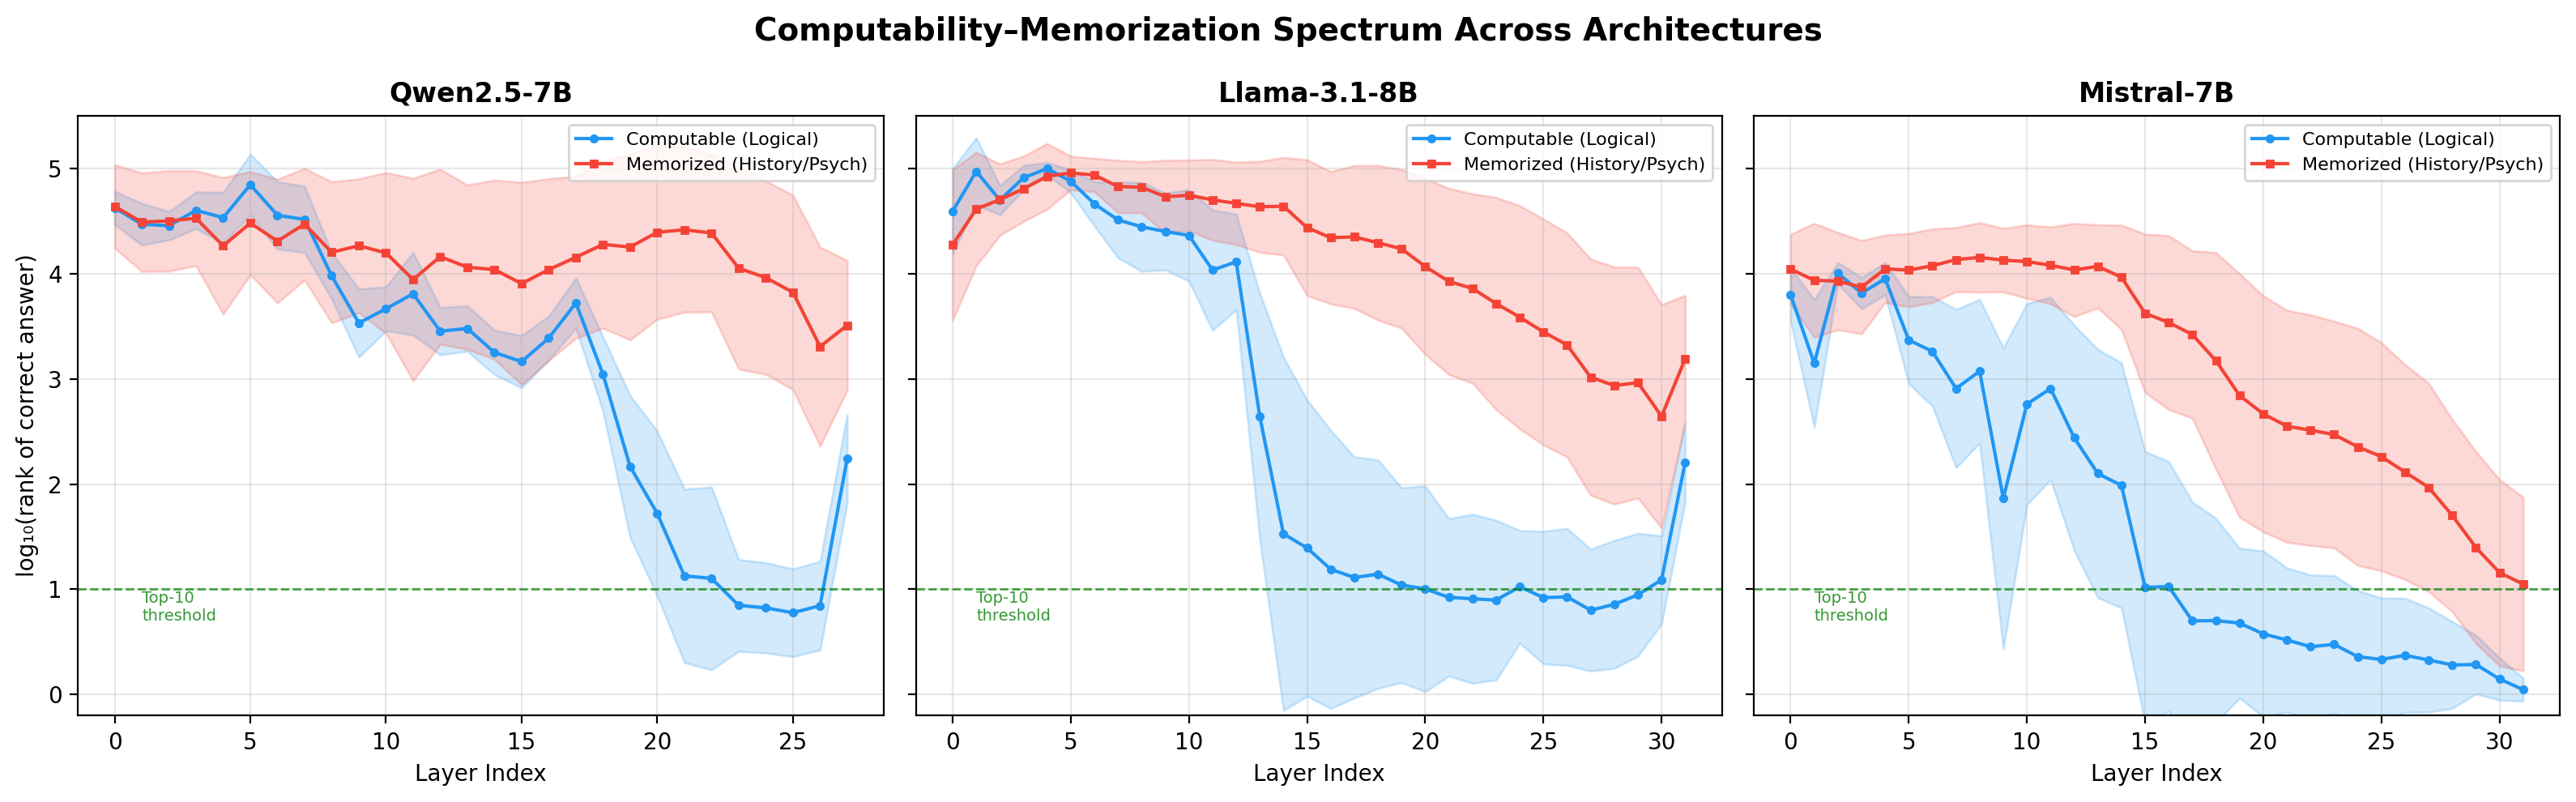
\includegraphics[width=\textwidth]{figures/computability_memorization_spectrum.png}
    \caption{Category-level FEP spectrum across architectures. Blue denotes categories treated as more computation-oriented (e.g., logical reasoning); red denotes fact-recall-heavy categories (e.g., history and psychology). These labels are descriptive proxies rather than controlled measures of computation or memorization.}
    \label{fig:spectrum}
\end{figure*}

\section{Top-$k$ Sensitivity Analysis}
\label{app:topk}

\begin{table}[htbp]
\centering\small
\begin{tabular}{rcccc}
\toprule
\textbf{$k$} & \textbf{Mean FEP} & \textbf{$\sigma$} & \textbf{Late Crystal} & \textbf{FEP Depth} \\
\midrule
1 & 28.0 & 0.0 & 100.0\% & 100.0\% \\
3 & 27.9 & 0.4 & 98.3\% & 99.8\% \\
5 & 27.6 & 1.4 & 92.9\% & 98.7\% \\
10 & 27.3 & 1.8 & 85.9\% & 97.5\% \\
20 & 27.0 & 2.1 & 80.2\% & 96.5\% \\
50 & 26.6 & 2.6 & 72.7\% & 95.0\% \\
100 & 26.0 & 3.4 & 64.7\% & 93.0\% \\
\bottomrule
\end{tabular}
\caption{FEP sensitivity to $k$ (Qwen2.5-7B, 817 samples). Late Crystallization is robust: even at $k{=}100$, 64.7\% of answers never appear at intermediate layers. FEP Depth stays $>$93\% across all thresholds.}
\label{tab:topk_sensitivity}
\end{table}

\section{Cross-Benchmark FEP Validation (MMLU)}
\label{app:mmlu}

\begin{table}[htbp]
\centering\small
\resizebox{\columnwidth}{!}{
\begin{tabular}{lccc}
\toprule
\textbf{Benchmark} & \textbf{$n$} & \textbf{Mean FEP} & \textbf{Late Crystal} \\
\midrule
TruthfulQA & 817 & 27.3$\pm$1.8 & 85.9\% \\
MMLU (all) & 1{,}200 & 27.9$\pm$0.5 & 98.2\% \\
\midrule
\quad STEM & 450 & 28.0$\pm$0.4 & 99.1\% \\
\quad Humanities & 250 & 28.0$\pm$0.4 & 98.0\% \\
\quad Social Sciences & 250 & 27.9$\pm$0.7 & 97.2\% \\
\quad Other & 250 & 27.9$\pm$0.6 & 98.0\% \\
\bottomrule
\end{tabular}
}
\caption{Cross-benchmark FEP validation (Qwen2.5-7B). Late Crystallization is even more pronounced on MMLU (98.2\%) than TruthfulQA (85.9\%), and consistent across all MMLU subject groups (97.2--99.1\%).}
\label{tab:mmlu_fep}
\end{table}

\section{Computability--Memorization Spectrum Details}
\label{app:spectrum}

Figure~\ref{fig:spectrum} visualizes category-level FEP across three architectures. Categories span a wide range: Logical Falsehood has the earliest mean FEP (22.1, $\sigma$=2.6), while History, Psychology, and Weather have FEP=28.0 with zero variance in this sample. The same ordering appears across Qwen2.5-7B, Llama-3.1-8B, and Mistral-7B. Because the category labels are only proxies and differ in content and difficulty, this descriptive gradient does not isolate computation from memorization. It motivates controlled follow-up work on whether category-conditioned interventions can improve high-FEP cases without disrupting earlier-emerging answers. Full per-category FEP statistics are available upon request.

\end{document}
